\documentclass[a4paper,12pt]{article}
\usepackage{amsmath,amsfonts,amsthm,amscd,amssymb,latexsym}%,eufrak}
%%%%%%%%%%%%%
\usepackage{caption}
\usepackage{subcaption}
\usepackage{enumerate,graphicx,psfrag}%,subfigure}%,jchangebar,oldgerm}
\usepackage[mathscr]{eucal}
\usepackage[usenames]{color}
\usepackage{url}
\usepackage[shortlabels]{enumitem}
\usepackage{comment}
%\usepackage[utf8]{inputenc}
\usepackage[T1]{fontenc}
%\usepackage{showkeys}
\usepackage{wrapfig}
\usepackage{lscape}
\usepackage{rotating}
%%%%%%%%%
\sloppy
%%%%%%%%%%%%%%%%%%%%%%%
\title{The subgroup membership problem in amalgamated products of 
finitely generated free groups
}
\author{Andrew J. Duncan, Elizaveta Frenkel}

\renewcommand{\a}{\alpha }
\renewcommand{\b}{\beta }
\newcommand{\G}{\Gamma }
\newcommand{\g}{\gamma }
\newcommand{\D}{\Delta }
\renewcommand{\d}{\delta }
%\def\vd{\vardelta}
\newcommand{\ep}{\epsilon }
\newcommand{\e}{\varepsilon }
\newcommand{\z}{\zeta }
%\eta
\renewcommand{\th}{\theta }
\newcommand{\T}{\Theta }
\renewcommand{\i}{\iota }
\renewcommand{\k}{\kappa }
\renewcommand{\l}{\lambda }
\renewcommand{\L}{\Lambda }
%\mu
%\nu
%\xi
%omicron
%\pi
\renewcommand{\r}{\rho }
\newcommand{\s}{\sigma }
\renewcommand{\S}{\Sigma }
\renewcommand{\t}{\tau }
\newcommand{\up}{\upsilon }
\newcommand{\U}{\Upsilon }
%\phi
\newcommand{\x}{\chi }
%\psi
\newcommand{\W}{\Omega }
\newcommand{\w}{\omega }
%%%%%%%%%%%%%%%%%%%%%%%%%%%%%%%
%%%%%%%%%%%%%%%%%%%%%%%%%%%%%
\newcommand{\pd}{\partial}
\newcommand{\wht}{\widehat}
%\newcommand{\cC}{{\mathcal C}}
%\newcommand{\cdim}{\texttt{cdim}}
\newcommand{\fC}{{\textswab C}}
\newenvironment{ef}{\noindent\color{blue} \bf EF: }{}
%
\newcommand{\cA}{{\cal{A}}}
\newcommand{\cD}{{\cal{D}}}
\newcommand{\cF}{{\cal{F}}}
\newcommand{\cH}{{\cal{H}}}
\newcommand{\cJ}{{\cal{J}}}
\newcommand{\cK}{{\cal{K}}}
\newcommand{\cP}{{\cal{P}}}
\newcommand{\cQ}{{\cal{Q}}}
\newcommand{\cR}{{\cal{R}}}
\newcommand{\cS}{{\cal{S}}}
\newcommand{\cV}{{\cal{V}}}
\newcommand{\cW}{{\cal{W}}}
%\newcommand{\GG}{\ensuremath{\mathbb{G}}}
\newcommand{\pp}{\mathbf{p}}
%%%%%%%%%%%%%%%%%%%%%%%%%%%%%%
\newcommand{\nul}{\emptyset }
\newcommand{\vim}{\nu\textrm{-im}}
%%%%%%%%%%%%%%%%%%%%%%%%%%%%%%
\newtheorem{theorem}{Theorem}[section]
\newtheorem{lemma}[theorem]{Lemma}
\newtheorem{corollary}[theorem]{Corollary}
\newtheorem{proposition}[theorem]{Proposition}
\newtheorem{axiom}[theorem]{Axiom}
\newtheorem{definition}[theorem]{Definition}
\newtheorem*{defn*}{Definition}
\newtheorem{conjecture}[theorem]{Conjecture}
%cvs -d :pserver:najd2@cvs.mas.ncl.ac.uk:/CVS/najd2
\newtheorem{exam}[theorem]{Example}
%\newtheorem{comment}[theorem]{Comment}
%
%
\newenvironment{example}{\begin{exam} \rm}{\end{exam}}
%
%
%
\newtheorem{remk}[theorem]{Remark}
\newenvironment{remark}{\begin{remk} \rm}{\end{remk}}
%
%%%%%%%%%%%%
\numberwithin{equation}{section}
\numberwithin{figure}{section}
%%%%%%%%%%%%%%%%%%%%
\newcommand{\Loop}{\operatorname{Loop}}
\newcommand{\Iso}{\operatorname{Isom}}
\newcommand{\Aut}{\operatorname{Aut}}
%%%%%%%%%%%%%%%%%%%
\renewcommand{\AA}{\ensuremath{\mathbb{A}}}
\newcommand{\ZZ}{\ensuremath{\mathbb{Z}}}
\newcommand{\QQ}{\ensuremath{\mathbb{Q}}}
\newcommand{\RR}{\ensuremath{\mathbb{R}}}
\newcommand{\NN}{\ensuremath{\mathbb{N}}}
\newcommand{\CC}{\ensuremath{\mathbb{C}}}
\newcommand{\FF}{\ensuremath{\mathbb{F}}}
%\renewcommand{\ker}{\verb"Ker"}
\newcommand{\cC}{\mathcal{C}}
\renewcommand{\cF}{\mathcal{F}}
\newcommand{\cO}{\mathcal{O}}
\renewcommand{\cS}{\mathcal{S}}
\newcommand{\la}{\langle}
\newcommand{\ra}{\rangle}
%\newcommand{\BA}{\ensuremath{\mathbb{A}}}
%%%%%%%%%%%%%%%%%%%%%%%%%%%%%%%%%%%%%%
\newcommand{\maps}{\rightarrow}
\newcommand{\ov}[1]{\overline{#1}}
\newcommand{\bs}{\backslash}
%%%%%%%%%%%%%%%%%%%%%%%%%%%%%%%
\newcommand{\be}{\begin{enumerate}}
\newcommand{\ee}{\end{enumerate}}
\newcommand{\bd}{\begin{description}}
\newcommand{\ed}{\end{description}}
\newcommand{\biz}{\begin{itemize}}
\newcommand{\eiz}{\end{itemize}}
%%%%%%%%%%%%%%%%%%%%%%%%%%%%%%%%%%%
%
\newenvironment{ajd1}{\noindent\color{red} AJD }{}
\newcommand{\ajd}[1]{\begin{ajd1} #1 \end{ajd1}}
%
%\includecomment{comp}% to see environment comp
\excludecomment{comp}% to hide environment comp
%
\begin{document}
\begin{example}\label{ex:f_1}
Let $F_1$ be the free group on generators $x_1,y_1$ and $H_1$ its
subgroup $H_1=\la
h_1,h_2,h_3, h_4\ra$, where  $h_1= x_1^3$, $h_2=y_1^{3}$, 
$h_3=x_1y_1^{3}x_1^{-1}$ and $h_4=x_1^{2}y_1^{3}x_1^{-2}$. 

The Stallings automata, $\G_{A_1}$ for $H_1$,
with maximal subtree $T_1$ highlighted and base vertex $1$, is shown
in Figure \ref{fig:bez1}.
The set $L_{T_1}$ corresponding to the maximal subtree  $T_1$ is
 $L_{T_1}=\{1,x_1,x_1^{2},y_1, y_1^2, x_1y_1, x_1y_1^2, x_1^2y_1, x_1^2y_1^2 \}$.

Let the set of double coset representatives for $H_1$ be $S_1=S_1^{(1)}
\cup S_1^{(2)}$.
To find the double coset normal form for the element $f_1 =
y_1^6 x_1^4 y_1 x_1^4 y_1 x_1^{-2} y_1^{-3} x_1^{-1}$: 
in
the notation of Algorithm I, use
${A_1}$ to read off the maximal acceptable prefix 
$h=y_1^6 x_1^3=h_2^2h_1$ 
of $f_1$; and
the maximal $L_{Q_1}$ prefix $p=x_1y_1$, of the remaining part of $f_1$. Next
$q^{-1}=x_1y_1^3x_1^2y_1^{-1}x_1^{-4}$, which has maximal acceptable prefix
$g=x_1y_1^3x_1^2=h_3h_1$. The maximal $L_{Q_1}$-prefix of the remaining part of $q^{-1}$
is then $t=y_1^{-1}$. Setting $e=x_1^4$,
\[f_1=h\circ p\circ e\circ t^{-1}\circ g^{-1}.\]
As $p$ is an $L_{T_1}$-prefix of $pq$ we have $y=p$. On the other hand
$t$ is not an $L_{T_1}$-prefix of $q^{-1}$ and $\t(t)=5$, so $z=w(5)=y_1^{2}$.
Now set
\[s=p\circ e\circ z^{-1}=x_1y_1x_1^4y_1^{-2}.\]
Then, writing $h^\prime=gtz^{-1}=h_3h_1h_2^{-1}$, the normal form for $f_1$ is
\[f_1=hs(h^\prime)^{-1}=(h_2^{2}h_1)x_1y_1x_1^4y_1^{-2} (h_2h_1^{-1}h_3^{-1})\in H_1S_1^{(1)}H_1.\]

To find the double coset normal form for the element
$f_2=y_1^3x_1^2y_1^3x_1^{-2}y_1^{-1}x_1y_1^{2}x_1^5$: use
${A_1}$ to read off the maximal acceptable prefix 
  $h=y_1^3x_1^2y_1^3x_1^{-2}=h_2h_4$ of $f_2$;   and 
the maximal $L_{Q_1}$-prefix 
$p=y_1^{-1}$, 
of the remainder of $f_2$.
  Here 
$q^{-1}=x_1^{-5}y_1^{-2}x_1^{-1}$, which has maximal acceptable prefix 
$g=x_1^{-3}=h_1^{-1}$ and the maximal $L_{Q_1}$-prefix of the remainder
 of $q^{-1}$ is then $t=x_1^{-2}y_1^{-2}x_1^{-1}$. Then $\t(p)=5$ so $y=w(5)=y_1^2$ and 
$\t(t)=$
\[f_2=p.\]
Therefore $f_2$ is in $H_1S_1^{(2)}H_1$. To find the required
double coset representative we construct $\G_{A_1}\times
\G_{A_1}$, which has two non-diagonal components of $9$ vertices, shown in Figure \ref{fig:bez1} and $18$ non-diagonal components of $3$ vertices, of
which $3$ are shown in Figure \ref{fig:bez2}. In these figures 
$\sim$ representatives are  
shown as
solid vertices and  connecting elements are the labels of paths in the
highlighted subtrees.  
Now, $u=\t(p)=6$ and $v=t=1$ so $\t(t)=1$ and $(6,1)$  is a 
 $\sim$ representative. 
 Therefore $y=p$, $z=1$,
$p=yz^{-1}\in S_1^{(2)}$, 
\[a=hpcy^{-1}=
\textrm{ and } b=zc^{-1}t^{-1}g^{-1}=x_1 x_2 x_2^{-1} x_1^{-1}=1,\]
and the normal form of $f_2$ is
\[f_2=a yz^{-1} b=(h_3^{-1}h_2) x_1^{-1}\in H_1S_1^{(2)}H_1.\]
\end{example}

\begin{figure}
\begin{center}
\psfrag{x1}{$x_1$}
\psfrag{y1}{$y_1$}
\psfrag{1}{$1$}
\psfrag{2}{$2$}
\psfrag{3}{$3$}
\psfrag{4}{$4$}
\psfrag{5}{$5$}
\psfrag{6}{$6$}
\psfrag{7}{$7$}
\psfrag{8}{$8$}
\psfrag{9}{$9$}
\subfigure[Stallings automaton $\G_{A_1}$ for $H_1$]{
\includegraphics[scale=.52]{bez1.eps}
\label{fig:bez1}}
\hspace{5mm}
\subfigure[$\G_{A_1}\times \G_{A_1}$: connected component of $(3,1)$.]{
\psfrag{x1}{$x_1$}
\psfrag{y1}{$y_1$}
\psfrag{1}{$(1,2)$}
\psfrag{2}{$(2,3)$}
\psfrag{3}{$(3,1)$}
\psfrag{4}{$(4,6)$}
\psfrag{5}{$(5,7)$}
\psfrag{6}{$(6,8)$}
\psfrag{7}{$(7,9)$}
\psfrag{8}{$(8,4)$}
\psfrag{9}{$(9,5)$}
\includegraphics[scale=.52]{bez1a.eps}
\label{fig:GxG-1}}
\hspace{5mm}
\subfigure[$\G_{A_1}\times \G_{A_1}$: connected component of $(2,1)$.]{
\psfrag{x1}{$x_1$}
\psfrag{y1}{$y_1$}
\psfrag{1}{$(1,3)$}
\psfrag{2}{$(2,1)$}
\psfrag{3}{$(3,2)$}
\psfrag{4}{$(4,8)$}
\psfrag{5}{$(5,9)$}
\psfrag{6}{$(6,4)$}
\psfrag{7}{$(7,5)$}
\psfrag{8}{$(8,6)$}
\psfrag{9}{$(9,7)$}
\includegraphics[scale=.52]{bez1b.eps}
\label{fig:GxG-2}}
\end{center}
\caption{Example \ref{ex:f_1}.}\label{fig:bez}
\end{figure}

\begin{figure}
\begin{center}
\subfigure[$\G_{A_1}\times \G_{A_1}$: connected component of $(6,1)$.]{
\psfrag{x1}{$x_1$}
\psfrag{y1}{$y_1$}
\psfrag{3}{$(6,1)$}
\psfrag{8}{$(7,4)$}
\psfrag{9}{$(2,5)$}
\includegraphics[scale=.52]{bez1c.eps}
\label{fig:GxG-18}}
\hspace{5mm}
\psfrag{x1}{$x_1$}
\psfrag{y1}{$y_1$}
\psfrag{3}{$(4,2)$}
\psfrag{8}{$(5,6)$}
\psfrag{9}{$(1,7)$}
\subfigure[$\G_{A_1}\times \G_{A_1}$: connected component of $(4,2)$.]{
\includegraphics[scale=.52]{bez1c.eps}
\label{fig:GxG-4}}
\hspace{5mm}
\subfigure[$\G_{A_1}\times \G_{A_1}$: connected component of $(9,3)$.]{
\psfrag{x1}{$x_1$}
\psfrag{y1}{$y_1$}
\psfrag{3}{$(9,3)$}
\psfrag{8}{$(3,8)$}
\psfrag{9}{$(8,9)$}
\includegraphics[scale=.52]{bez1c.eps}
\label{fig:GxG-5}}
\end{center}
\caption{Example \ref{ex:f_1}.}\label{fig:bez2}
\end{figure}

\begin{example}\label{ex:f_2}
Let $F_2$ be the free group on generators
$y_1,y_2,y_3,y_4$ with a subgroup $H_2 = \la h_1^{\prime},
h_2^{\prime},h_3^{\prime}\ra$, where
$h_1^{\prime}=y_2^2$,
$h_2^{\prime}=y_3y_4$ and
$h_3^{\prime}=y_1^2y_3y_1^{-1}y_2$.
The Stallings automata, $\G_{A_2}$ for $H_2$,
with maximal subtree $T_2$ highlighted and base vertex $1$, is shown
in Figure \ref{fig:stallagain}.\ref{fig:stallh2}.
The set $L_{T_2}$ corresponding to the maximal subtree  $T_2$ is
 $L_{T_2}=
\{1, y_1, y_1^2,
y_2^{-1}, y_2^{-1}y_1, y_3 \}$.
Let the set of double coset representatives for $H_2$ be $S_2=S_2^{(1)}
\cup S_2^{(2)}$.

To find the normal form of $f_1^\prime=y_1^2y_3y_1^{-1}y_2y_3y_4y_1y_2
y_3y_4y_2^2$: use ${A_2}$ to read off the maximal acceptable
prefix $h= y_1^2y_3y_1^{-1}y_2y_3y_4$ of $f_1^\prime$; and  the maximal
$L_{Q_2}$-prefix $p=y_1$ of the rest of $f_1^\prime$.  Next $q^{-1}=
y_2^{-2}y_4^{-1}y_3^{-1}y_2^{-1}$, so $g=y_2^{-2}y_4^{-1}y_3^{-1}$
and $t=y_2^{-1}$. This element will be represented by an element
of $S_2^{(2)}$, so we need to construct $\G_{A_2}\times \G_{A_2}$.
There are $7$  non-trivial, non-diagonal components. One is shown
in Figure \ref{fig:stallagain}\ref{fig:G2xG2-1} and the remaining
six in Figure \ref{fig:G2xG2-2}. In all cases the solid vertex
corresponds to the $\sim$ representative and connecting elements
are paths in the highlighted trees. Following Algorithm I, the
normal form of $f_1^\prime$ is seen to be
\[f_1^\prime=h yz^{-1} g^{-1},\]
where $y=y_1$, $z=y_2$ and $yz^{-1}=y_1y_2^{-1}\in S_2^{(2)}$: that is
\[f_1^\prime=h^\prime_3h_2^\prime y_1y_2^{-1} (h_1^\prime)^{-1}(h_2^\prime)^{-1}.\]
\end{example}

\begin{figure}
\begin{center}

\psfrag{y1}{$y_1$}

\psfrag{y2}{$y_2$}

\psfrag{y3}{$y_3$}

\psfrag{y4}{$y_4$}
\psfrag{1}{$1$}
\psfrag{2}{$2$}
\psfrag{3}{$3$}
\psfrag{4}{$4$}
\psfrag{5}{$5$}
\psfrag{6}{$6$}
\subfigure[Stallings automaton $A_2$ for $H_2$]{
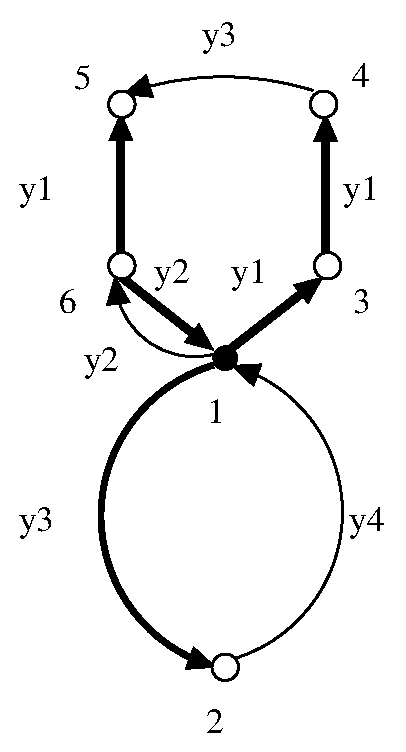
\includegraphics[scale=.52]{stallh2.eps}
\label{fig:stallh2}}
\hspace{25mm}
\subfigure[$\G_{A_2}\times \G_{A_2}$: connected component of
$(6,1)$.]{
\psfrag{a}{$(5,3)$}
\psfrag{b}{$(6,1)$}
\psfrag{c}{$(1,6)$}
\psfrag{d}{$(3,5)$}
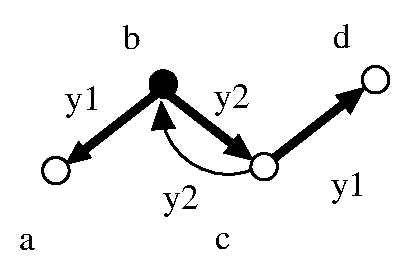
\includegraphics[scale=.52]{G2xG2-1.eps}
\label{fig:G2xG2-1}}
\end{center}
\caption{Stallings automata for Example \ref{ex:f_2}.}\label{fig:stallagain}
\end{figure}

\begin{figure}
\begin{center}

\psfrag{y1}{$y_1$}

\psfrag{y2}{$y_2$}

\psfrag{y3}{$y_3$}

\psfrag{y4}{$y_4$}
\psfrag{b}{$(1,3)$}
\psfrag{c}{$(3,4)$}
\subfigure[$(1,3)$.]{
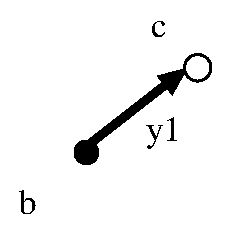
\includegraphics[scale=.5]{G2xG2-2.eps}
\label{fig:G2xG2-2-1}}
\hspace{1mm}
\subfigure[$(3,1)$.]{
\psfrag{b}{$(3,1)$}
\psfrag{c}{$(4,3)$}
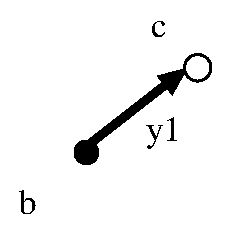
\includegraphics[scale=.5]{G2xG2-2.eps}
\label{fig:G2xG2-2-2}}
\hspace{1mm}
\subfigure[$(2,5)$.]{
\psfrag{y1}{$y_3$}
\psfrag{b}{$(1,4)$}
\psfrag{c}{$(2,5)$}
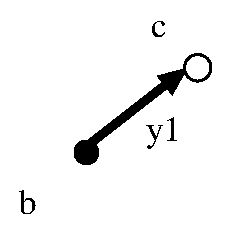
\includegraphics[scale=.5]{G2xG2-2.eps}
\label{fig:G2xG2-2-3}}
\hspace{1mm}
\subfigure[$(5,2)$.]{
\psfrag{y1}{$y_3$}
\psfrag{b}{$(4,1)$}
\psfrag{c}{$(5,2)$}
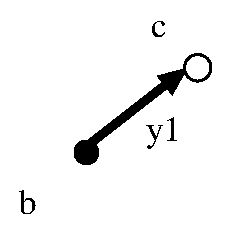
\includegraphics[scale=.5]{G2xG2-2.eps}
\label{fig:G2xG2-2-4}}
\hspace{1mm}
\subfigure[$(4,5)$.]{
\psfrag{y1}{$y_1$}
\psfrag{b}{$(3,6)$}
\psfrag{c}{$(4,5)$}
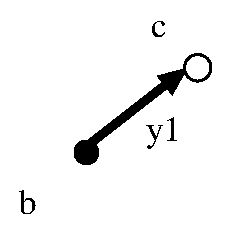
\includegraphics[scale=.5]{G2xG2-2.eps}
\label{fig:G2xG2-2-5}}
\hspace{1mm}
\subfigure[$(6,3)$.]{
\psfrag{b}{$(6,3)$}
\psfrag{c}{$(5,4)$}
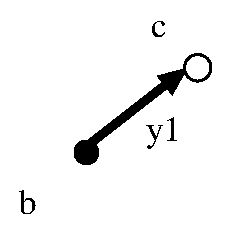
\includegraphics[scale=.5]{G2xG2-2.eps}
\label{fig:G2xG2-2-6}}
\end{center}
\caption{Example \ref{ex:f_2}: connected components of $\G_{A_2}\times \G_{A_2}$.}\label{fig:G2xG2-2}
\end{figure}
\end{document}